% CadQuarry: a permissively-licensed, procedurally-generated parametric CAD dataset.
% Compile: latexmk -lualatex -shell-escape main.tex   (requires biber + pygments)
\documentclass[11pt]{article}

% ---------------------------------------------------------------------------
% Page geometry & encoding
% ---------------------------------------------------------------------------
\usepackage[a4paper,margin=1in,headsep=14pt]{geometry}
\usepackage{fontspec}
\usepackage{unicode-math}
\usepackage{microtype}

% Libertinus for text + math, Source Code Pro for code. All ship with TeX Live.
\setmainfont{LibertinusSerif}[
  Extension      = .otf,
  UprightFont    = *-Regular, ItalicFont = *-Italic,
  BoldFont       = *-Semibold, BoldItalicFont = *-SemiboldItalic ]
\setsansfont{LibertinusSans}[
  Extension      = .otf,
  UprightFont    = *-Regular, ItalicFont = *-Italic, BoldFont = *-Bold ]
\setmonofont{SourceCodePro}[
  Extension      = .otf,
  UprightFont    = *-Regular, BoldFont = *-Semibold, Scale = 0.88 ]
\setmathfont{LibertinusMath-Regular.otf}

% ---------------------------------------------------------------------------
% Colour palette (keyed off the renderer's matte-blue CAD look)
% ---------------------------------------------------------------------------
\usepackage[table]{xcolor}
\definecolor{ink}{HTML}{1B2436}      % near-black slate, body emphasis
\definecolor{accent}{HTML}{3F6FD1}   % primary blue
\definecolor{accentd}{HTML}{2A4E9B}  % darker blue
\definecolor{accent2}{HTML}{C2410C}  % warm secondary (threads/gears)
\definecolor{rule}{HTML}{C9D2E3}     % light divider
\definecolor{panel}{HTML}{F3F6FC}    % pale panel fill
\definecolor{panel2}{HTML}{FBF4EE}   % warm panel fill
\definecolor{codebg}{HTML}{F7F8FB}
\definecolor{good}{HTML}{1F7A4D}

% ---------------------------------------------------------------------------
% Graphics, tables, lists
% ---------------------------------------------------------------------------
\usepackage{graphicx}
\usepackage{booktabs}
\usepackage{tabularx}
\usepackage{array}
\usepackage{multirow}
\usepackage{enumitem}
\setlist{noitemsep,topsep=2pt,leftmargin=1.35em}
\usepackage{fontawesome5}
\usepackage{pifont}

\usepackage{caption}
\captionsetup{font={small,sf},labelfont={bf,color=accentd},labelsep=period,
  width=.95\linewidth}

% ---------------------------------------------------------------------------
% TikZ + pgfplots
% ---------------------------------------------------------------------------
\usepackage{tikz}
\usetikzlibrary{arrows.meta,positioning,shapes.geometric,fit,backgrounds,calc,decorations.pathreplacing}
\usepackage{pgfplots}
\pgfplotsset{compat=1.18}
\usepgfplotslibrary{colorbrewer}

% ---------------------------------------------------------------------------
% Callout boxes
% ---------------------------------------------------------------------------
\usepackage[skins,breakable]{tcolorbox}
\newtcolorbox{keybox}[1][]{
  enhanced, breakable, colback=panel, colframe=accent,
  boxrule=0pt, leftrule=2.5pt, arc=2pt, left=10pt, right=10pt, top=7pt, bottom=7pt,
  coltitle=white, fonttitle=\sffamily\bfseries, title={#1} }
\newtcolorbox{warnbox}[1][]{
  enhanced, breakable, colback=panel2, colframe=accent2,
  boxrule=0pt, leftrule=2.5pt, arc=2pt, left=10pt, right=10pt, top=7pt, bottom=7pt,
  coltitle=white, fonttitle=\sffamily\bfseries, title={#1} }

% ---------------------------------------------------------------------------
% Code listings (minted v3 + pygments)
% ---------------------------------------------------------------------------
\usepackage{minted}
\usemintedstyle{friendly}
\setminted{
  fontsize=\footnotesize, breaklines=true, autogobble=true,
  bgcolor=codebg, frame=none, tabsize=2, framesep=2mm }
\setminted[python]{python3=true}

% ---------------------------------------------------------------------------
% Section styling
% ---------------------------------------------------------------------------
\usepackage{titlesec}
\titleformat{\section}{\sffamily\large\bfseries\color{ink}}
  {\color{accent}\thesection}{0.6em}{}
\titleformat{\subsection}{\sffamily\normalsize\bfseries\color{accentd}}
  {\thesubsection}{0.5em}{}
\titlespacing*{\section}{0pt}{1.4ex plus .3ex minus .2ex}{0.7ex}
\titlespacing*{\subsection}{0pt}{1.0ex plus .2ex}{0.4ex}

% Header rule
\usepackage{fancyhdr}
\pagestyle{fancy}\fancyhf{}
\renewcommand{\headrulewidth}{0.4pt}
\renewcommand{\footrulewidth}{0pt}
\fancyhead[L]{\sffamily\footnotesize\color{ink}CadQuarry}
\fancyhead[R]{\sffamily\footnotesize\color{ink}A Procedurally-Generated Parametric CAD Dataset}
\fancyfoot[C]{\sffamily\footnotesize\thepage}

% ---------------------------------------------------------------------------
% References
% ---------------------------------------------------------------------------
\usepackage[backend=biber,style=numeric-comp,sorting=none,giveninits=true,
  maxbibnames=8,url=true,doi=false,isbn=false]{biblatex}
\addbibresource{references.bib}
\renewcommand*{\bibfont}{\small}

\usepackage[colorlinks=true,allcolors=accentd,breaklinks=true]{hyperref}
\usepackage[nameinlink,capitalise]{cleveref}

% Small helpers. \code is plain monospace (Source Code Pro): its arguments are
% already LaTeX-escaped, and using \texttt rather than \mintinline{text} avoids
% 65 needless Pygments shell-outs (and minted v3's cold-cache rerun errors).
\newcommand{\code}[1]{\texttt{#1}}
\newcommand{\fm}[1]{\textsf{\small #1}}
\newcommand{\cc}{\textsc{cc0-1.0}}
\newcommand{\apache}{Apache-2.0}

% ===========================================================================
\begin{document}
% ===========================================================================

\thispagestyle{empty}
\begin{center}
  {\sffamily\bfseries\fontsize{21}{25}\selectfont\color{ink}
   CadQuarry: A Permissively-Licensed,\\[2pt]
   Procedurally-Generated Dataset of Parametric CAD Programs}\\[10pt]
  {\large Jacob Jennings}\\[2pt]
  {\small Independent Researcher \;\textbar\; \href{mailto:jacob.r.jennings@gmail.com}{jacob.r.jennings@gmail.com}}\\[3pt]
  {\small\sffamily
    \faGithub\;\href{https://github.com/jacobjennings/CadQuarry}{github.com/jacobjennings/CadQuarry}
    \quad\textbar\quad
    \faDatabase\;\href{https://huggingface.co/datasets/jacobjennings/cadquarry}{huggingface.co/datasets/jacobjennings/cadquarry}}\\[4pt]
  {\footnotesize Code: \apache{} \;\textbar\; Data: \cc{} (public domain) \;\textbar\; \today}
\end{center}
\vspace{2pt}

% ---- Teaser ----------------------------------------------------------------
\begin{figure}[h]
  \centering
  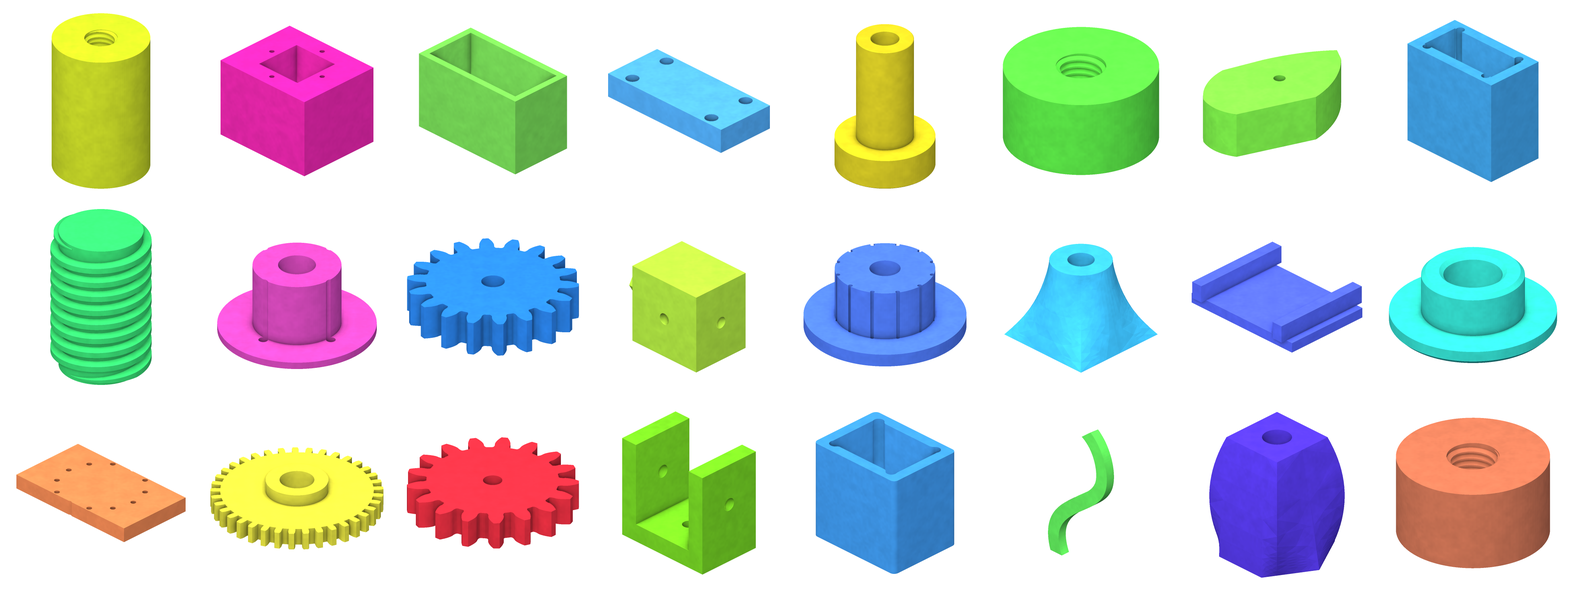
\includegraphics[width=\linewidth]{figures/teaser.png}
  \caption{A 24-part sample drawn across CadQuarry's fifteen part families. Every
  object is a deterministic function of a single integer seed, executes to a
  watertight solid, and ships as live-editable parametric CadQuery code under a
  \cc{} public-domain dedication. Images are CadQuarry's own headless GPU
  renders (\cref{sec:render}).}
  \label{fig:teaser}
\end{figure}

% ---- Abstract --------------------------------------------------------------
\begin{tcolorbox}[enhanced,colback=white,colframe=rule,boxrule=0.5pt,arc=2pt,
  left=12pt,right=12pt,top=8pt,bottom=8pt]
\noindent\textbf{\sffamily\color{ink}Abstract.}\;
Progress on learning-based CAD generation is gated by data whose licensing is
restrictive or ambiguous and whose programs are fixed instances rather than
editable designs. We present \textbf{CadQuarry}, a procedural generator and the
corpus it produces: diverse, executable, \emph{parametric} CadQuery programs
released as public-domain (\cc{}) data with an \apache{} generator. Each part is
a typed parameter schema plus a pure \code{build(p)} function, so any sample is a
live design whose geometry updates in milliseconds, not a frozen mesh. The
vocabulary spans plates, brackets, shafts, blocks, multi-section assemblies,
freeform 2D sketches (line/arc/B\'ezier/spline loops, extruded or revolved),
lofted reducers, swept profiles, and three solver-built mechanical
families---involute/cycloid \emph{gears}, standards-based \emph{threads}
(ISO/ACME/trapezoidal), and \emph{tapped} holes with real cut internal
threads---raising the complexity ceiling beyond the fixed sketch-extrude
sequences of prior corpora. Validity is guaranteed by execution
and duplicates are removed by a rotation/translation-invariant geometry
signature; across our largest corpus all 200{,}000 accepted parts are
geometrically distinct. The data is published on the Hugging Face Hub as a size
ladder (1k--200k) in six content configs---code-only JSONL plus Parquet with
binary STEP, STL, and eight-view GPU renders---and is browsable through a
committed in-browser gallery, and any corpus can be regenerated from a versioned
seed list. Generation sustains \mbox{$\sim$10} validated parts/s on a 24-core
workstation, paced by the solver-built mechanical families.
\end{tcolorbox}

% ===========================================================================
\section{Introduction}
% ===========================================================================
Data-driven CAD---generating, completing, or recovering parametric solid models
with neural networks---has advanced quickly, but the field's datasets carry two
practical frictions.

\textbf{Licensing.} Today's CAD datasets are, almost without exception, either
non-commercial or bound by unsettled per-model terms. The large collected
corpora---ABC~\cite{abc} and the sketch-extrude sequences derived from it
(DeepCAD~\cite{deepcad} and its text-augmented descendant
Text2CAD~\cite{text2cad})---are parsed from Onshape public documents, so their
geometry stays copyright its creators under those source terms; the
human-authored Fusion~360 Gallery~\cite{fusion360} ships under a custom Autodesk
\emph{non-commercial} research license, and even the procedurally generated
CAD-Recode~\cite{cadrecode} is released CC~BY-NC. Unrestricted---especially
commercial---reuse is therefore a
case-by-case legal question rather than a settled fact (\cref{tab:compare}).

\textbf{Editability.} Most released CAD datasets are \emph{instances}: a fixed
construction sequence or B-rep for one shape. The closest analog to this work,
CAD-Recode~\cite{cadrecode}, takes the elegant step of representing each model as
CadQuery Python and procedurally generating a million of them---but those
programs likewise encode single, fixed sketch-extrude solids. A program that is
already a function of named, range-bounded parameters is strictly more useful: it
is a design, not a snapshot.

CadQuarry targets both frictions directly, and pushes on the complexity ceiling
while it does so.

\begin{keybox}[Contributions]
\begin{enumerate}[label=\textbf{\arabic*.}]
  \item A \textbf{procedural generator} (\apache{}) that emits diverse, valid,
        \emph{parametric} CadQuery programs, and the \textbf{corpus} it produces,
        released as public-domain \cc{} data---clean for any use, commercial
        included.
  \item \textbf{Parametric-by-construction} programs: a machine-readable
        \code{PARAMS} schema plus a pure \code{build(p)} function. Samples are
        live-editable designs, enabling research on customizable parts, data
        augmentation, and parameter inference.
  \item A \textbf{raised complexity ceiling}: freeform sketched profiles, lofts
        and sweeps, multi-section assemblies, and three solver-built mechanical
        families---involute/cycloid gears, standards-based threads, and tapped
        holes---bridged into a single CadQuery solid.
  \item \textbf{Validity by execution} and \textbf{geometry-signature dedup};
        empirically, 200{,}000/200{,}000 accepted parts are distinct.
  \item \textbf{Developer experience}: a Hugging Face size ladder in Parquet/JSONL
        configs, \textbf{eight-view} GPU renders, and a no-install in-browser
        gallery and live customizer.
  \item \textbf{An extensible generator built for a community}: because every
        corpus is a function of an \apache{} generator and a versioned seed list,
        a new family or an improved sampler is just a new generator
        version---inviting others to iterate on and grow the design space rather
        than re-scrape it, with no proprietary pipeline in the loop.
\end{enumerate}
\end{keybox}

% ===========================================================================
\section{Related CAD Datasets}\label{sec:related}
% ===========================================================================
\Cref{tab:compare} situates CadQuarry among widely used CAD datasets. We follow
the \emph{Datasheets for Datasets}~\cite{datasheets} framing: because our
contribution is the data and tooling rather than a model, the rest of the paper
is organized as a datasheet---generation methodology, validity characterization,
distribution statistics, intended uses, and licensing---rather than as a methods
paper. CAD-Recode~\cite{cadrecode} and Fusion~360 Gallery~\cite{fusion360} are
the closest references for framing generation and tasks; recent work such as
CADmium~\cite{cadmium} illustrates the geometric-quality evaluation our data is
meant to support.

\begin{table}[h]
\centering\small\setlength{\tabcolsep}{5pt}
\renewcommand{\arraystretch}{1.2}
\newcommand{\yes}{\textcolor{good}{\ding{51}}}
\newcommand{\no}{\textcolor{rule!60!ink}{\ding{55}}}
\begin{tabularx}{\linewidth}{@{}l r >{\raggedright\arraybackslash}X l c l@{}}
\toprule
\textbf{Dataset} & \textbf{Scale} & \textbf{Representation} & \textbf{Origin}
 & \textbf{Param.\textsuperscript{a}} & \textbf{Data license\textsuperscript{b}}\\
\midrule
ABC~\cite{abc}            & $\sim$1M   & B-rep (STEP)              & collected   & \no & Onshape ToU$^{\dagger}$\\
DeepCAD~\cite{deepcad}    & $\sim$178k & sketch-extrude seq.       & from ABC    & \no & Onshape ToU$^{\dagger}$\\
Fusion 360~\cite{fusion360}& 8{,}625   & seq.\ $+$ timeline         & human       & \no & non-comm.\ res.\\
Text2CAD~\cite{text2cad}  & $\sim$170k & seq.\ $+$ text             & aug.\ DeepCAD& \no & CC BY-NC-SA\\
CAD-Recode~\cite{cadrecode}& 1M        & CadQuery code (fixed)     & procedural  & \no & CC BY-NC\\
\rowcolor{panel}\textbf{CadQuarry} & up to 200k\textsuperscript{c} & \textbf{parametric CadQuery} $+$ B-rep, STL, renders & procedural & \yes & \textbf{\cc{}}\\
\bottomrule
\end{tabularx}
\caption{CadQuarry in context. \textsuperscript{a}\,Programs are functions of
named, range-bounded parameters (live-editable), not fixed instances.
\textsuperscript{b}\,Data license \emph{as published} (June 2026); verify at
source. $^{\dagger}$\,ABC and DeepCAD geometry is parsed from Onshape public
documents and remains copyright its creators under Onshape's Terms of Use---the
repositories' MIT license covers their code, not the models. Fusion~360 Gallery
is non-commercial research-only (no full redistribution); Text2CAD is
CC~BY-NC-SA~4.0; CAD-Recode's corpus is CC~BY-NC~4.0. CadQuarry is the only
public-domain (\cc{}) corpus here---the only one usable commercially with no
attribution. \textsuperscript{c}\,Published ladder; the generator is unbounded,
and any corpus is reproducible from its seed.}
\label{tab:compare}
\end{table}

\noindent The differentiators we foreground are not claimed elsewhere as primary
contributions: an unambiguous public-domain grant, live parametric editability,
and real mechanical geometry (threads, gears, assemblies) alongside the usual
prismatic and revolved parts.

% ===========================================================================
\section{Generation Pipeline}\label{sec:pipeline}
% ===========================================================================
CadQuarry samples an intermediate representation (IR), emits self-contained
CadQuery source, executes it in a sandbox, and accepts the part only if it builds
to a single valid solid that is not a geometric duplicate of one already seen
(\cref{fig:pipeline}). The IR, emitter, composer, and deduplicator have no
dependency on CadQuery itself; only execution does.

\begin{figure}[h]
\centering
\begin{tikzpicture}[
  font=\sffamily\scriptsize,
  node distance=5.5mm and 6mm,
  box/.style={draw=accent, fill=panel, rounded corners=2pt, align=center,
    inner sep=4pt, minimum height=8.5mm, text width=15mm},
  io/.style={draw=accentd, fill=white, rounded corners=2pt, align=center,
    inner sep=4pt, minimum height=8.5mm, text width=13mm},
  acc/.style={draw=good, fill=good!8, rounded corners=2pt, align=center,
    inner sep=4pt, minimum height=8.5mm, text width=14mm},
  arr/.style={-{Stealth[length=4.5pt]}, accentd, thick},
  lbl/.style={font=\sffamily\fontsize{6.2}{7}\selectfont, text=ink}]

\node[io] (seed) {\textbf{seed}\\ $+$ config};
\node[box, right=of seed] (sample) {sample\\ family $+$ tier};
\node[box, right=of sample] (ir) {compose\\ \textbf{IR}};
\node[box, right=of ir] (emit) {emit\\ \code{.py}};
\node[box, right=of emit] (exec) {execute\\ (sandbox)};
\node[box, right=of exec] (valid) {validate\\ $+$ dedup};
\node[acc, right=of valid] (acc) {\textbf{accept}};

\foreach \a/\b in {seed/sample, sample/ir, ir/emit, emit/exec, exec/valid, valid/acc}
  \draw[arr] (\a) -- (\b);

% reject feedback
\draw[arr, accent2, dashed] (valid.south) .. controls +(0,-7mm) and +(0,-7mm) .. (sample.south)
  node[midway, below, font=\sffamily\fontsize{6.2}{7}\selectfont, text=accent2]
  {reject (invalid / disconnected / duplicate) $\rightarrow$ resample};

% downstream
\node[io, below=10mm of acc, text width=20mm] (out)
  {\textbf{export}\\ STEP\,/\,STL\\ 8-view renders\\ point cloud};
\draw[arr] (acc) -- (out);
\node[io, left=8mm of out, text width=20mm] (pack)
  {\textbf{pack}\\ JSONL $+$ Parquet};
\draw[arr] (out) -- (pack);
\node[io, left=8mm of pack, text width=14mm] (hf)
  {\faDatabase\ Hugging\\ Face Hub};
\draw[arr] (pack) -- (hf);

\node[lbl, above=1pt of sample] {seeded RNG};
\node[lbl, above=1pt of exec] {persistent workers};
\end{tikzpicture}
\caption{The generation pipeline. Sampling is seeded per part and the
accept/reject decision is taken in strict attempt order, so the corpus is
identical regardless of how many workers run. Text artifacts (code,
params, meta) are produced by \code{generate}; geometry and renders are produced
on demand by \code{export}.}
\label{fig:pipeline}
\end{figure}

\subsection{Part families and complexity tiers}
Fifteen families span a deliberately broad operation vocabulary
(\cref{fig:families}). Twelve are self-contained on CadQuery alone; the three
mechanical families are described in \cref{sec:mech}. Each part also draws a
\emph{complexity tier} (0--3) that governs how many features it carries---from a
bare primitive (tier~0) to deep multi-section trees with pockets, bosses, ribs,
and extra ports (tier~3). Tiers are clamped per family (e.g.\ brackets and
assemblies start at tier~1), and the \fm{compound} family scales its section
count with tier, so a manifold sprouts additional bored ports as complexity
rises.

\begin{figure}[h]
\centering
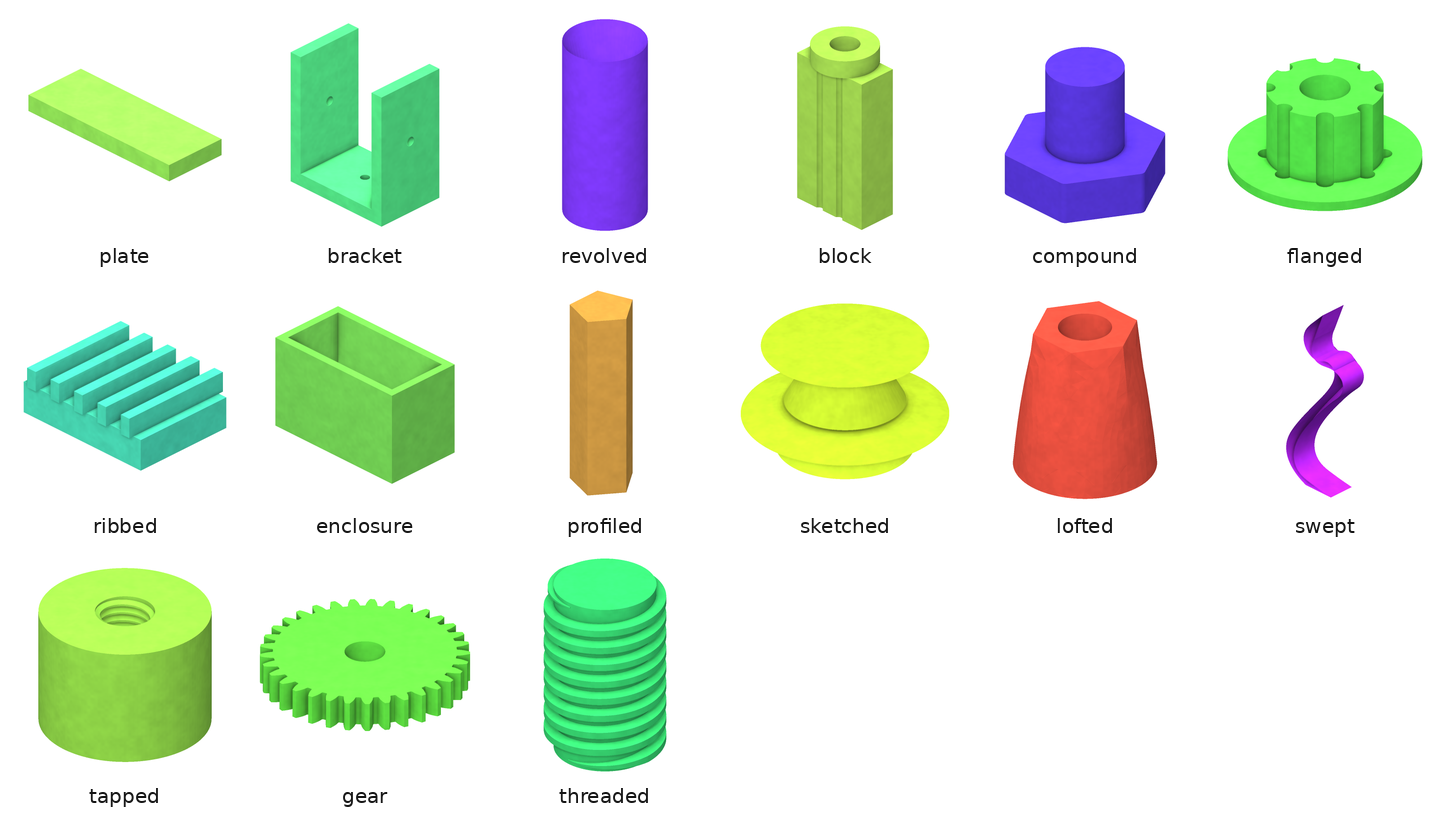
\includegraphics[width=\linewidth]{figures/families.png}
\caption{One representative per family (default parameters, \code{iso\_fr}
render). \fm{plate}, \fm{bracket} (L/C/Z angle brackets with gussets),
\fm{revolved} shafts/bushings, \fm{block} housings, \fm{compound}
multi-section assemblies, \fm{flanged} bolt-circle hubs, \fm{ribbed}
structures, shelled \fm{enclosure}s, \fm{profiled} bars, \fm{sketched}
freeform line/arc/B\'ezier/spline bodies, \fm{lofted} reducers, \fm{swept}
profiles, \fm{tapped} bodies, involute \fm{gear}s, and standards-based
\fm{threaded} parts.}
\label{fig:families}
\end{figure}

\subsection{Parametric program format}
Every emitted \code{.py} is self-contained and customizer-compatible: a typed,
range-bounded, UI-labeled \code{PARAMS} schema and a pure \code{build(p)} that is
a function of those parameters (\cref{fig:param}). This is the property that turns
a sample from a frozen instance into a \emph{design}---the same program yields a
continuum of valid parts, which is what makes the data useful for customizable-part
research, parameter inference, and on-the-fly augmentation. To be precise about
scope: each published record is one program materialized at its \emph{default}
parameters---the geometry, eight-view renders, and dimension summary all describe
the part \code{build(p)} produces under those defaults. We deliberately do
\emph{not} enumerate the combinatorial space of parameter settings into the
corpus; doing so would bloat it with near-duplicates and defeat dedup. The point
of shipping the \code{PARAMS} schema and the \code{build(p)} function is to invite
models to \emph{generate} parametric programs, not to pre-render every output of
one. A sidecar
\code{.params.json} mirrors the schema for consumers that do not execute Python,
and---for families with categorical design intent---a machine-readable
\code{descriptor} resolves the part's defining attributes (e.g.\ a thread's
\code{M16x2} designation, a gear's module and tooth count) so they can be queried
without parsing source. Every part additionally carries a procedurally-generated,
plain-English \emph{dimension summary}---a short, prompt-friendly description of
its overall size and each feature (holes, fillets, bores, pockets, brackets,
gears, threads), resolved against the default parameters. Crucially this is
\emph{not} AI-written text: it is a pure, deterministic walk of the IR (e.g.\
\textit{``Rectangular body, 55\,$\times$\,23.5\,$\times$\,75.4\,mm (W$\times$D$\times$H).
Four \O3.2\,mm holes at the corners, 38.5\,$\times$\,16.45\,mm spacing. Fillet
radius 1.078\,mm on vertical edges.''}), so it is deterministic and
pairs with the renders (\cref{sec:render}) as a faithful text--image signal for
captioning and program-recovery work. The summary is emitted as a
\code{dimensions} field in the metadata, a \code{dims/} text sidecar, and a column
of the published tables.

\begin{figure}[h]
\begin{minipage}[t]{0.585\linewidth}
\vspace{0pt}
\begin{minted}{python}
import cadquery as cq
# CadQuarry v0.6.0 - seed 1234003889 - CC0-1.0

PARAMS = {
  "base_len":  {"type": "float", "default": 60.0,
     "min": 25, "max": 90, "group": "Body",
     "label": "Base leg length (mm)"},
  "n_holes":   {"type": "int", "default": 2,
     "min": 1, "max": 3, "group": "Holes",
     "label": "Holes per leg"},
  "gusset":    {"type": "bool", "default": True,
     "group": "Gusset", "label": "Corner gusset"},
  # ... 5 more typed, range-bounded params
}

def build(p):
    base  = cq.Workplane("XY").box(
        p["base_len"], p["bracket_w"], p["bracket_t"],
        centered=(False, True, False))
    vert1 = cq.Workplane("XY").box(...)   # near leg
    vert2 = cq.Workplane("XY").box(...)   # far leg
    result = base.union(vert1).union(vert2)
    if p["gusset"]:
        result = result.union(...)        # corner gussets
    return result   # -> one watertight solid

result = build({k: v["default"]
                for k, v in PARAMS.items()})
\end{minted}
\end{minipage}\hfill
\begin{minipage}[t]{0.395\linewidth}
\vspace{6pt}
\centering
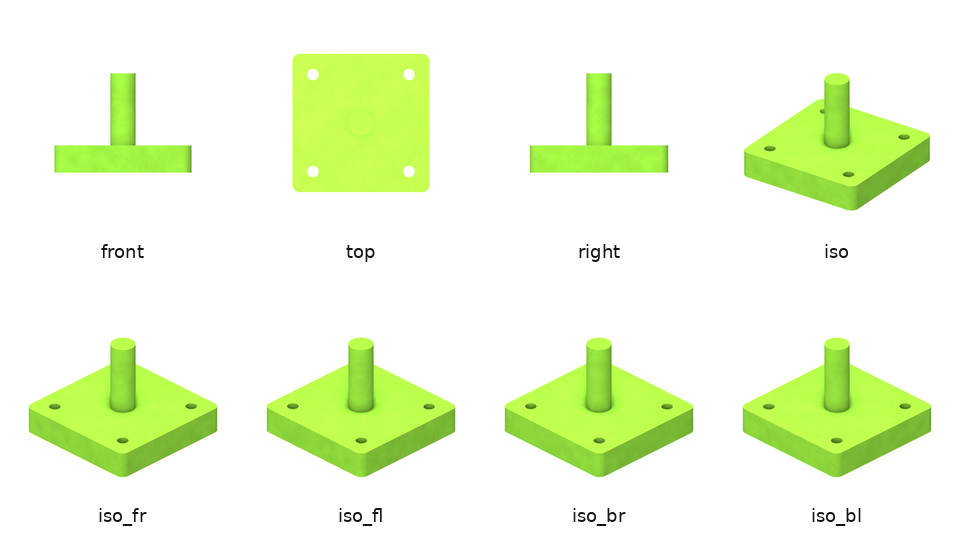
\includegraphics[width=\linewidth]{figures/eightview.png}\\[3pt]
{\footnotesize\sffamily The eight standard viewpoints of the part this program
builds at its default parameters: three orthographic (\code{front}/\code{top}/%
\code{right}), a canonical \code{iso}, and the four isometric corners.}
\end{minipage}
\caption{An abbreviated but faithful generated \fm{bracket} program (left) and
the eight-view render of the solid it produces (right). Moving any slider
re-runs \code{build} and updates all geometry; nothing is pre-baked.}
\label{fig:param}
\end{figure}

% ===========================================================================
\section{Validity, Deduplication, and Reproducibility}\label{sec:valid}
% ===========================================================================
\textbf{Validity by execution.} CadQuarry never ships a part it has not built. A
candidate is accepted only if its program runs to completion and yields exactly
\emph{one} connected solid of non-trivial volume, finite bounding box, and a
plausible aspect ratio; multiple solids signal a union that failed to fuse and
are rejected. This trades a little yield for the guarantee that every published
program executes.

\textbf{Geometry-signature dedup.} To avoid near-trivial repeats, each solid is
reduced to a signature of quantized, analytically computed invariants:

\vspace{-2pt}
\[
\sigma \;=\; \big(\,V,\; A,\; \mathrm{sort}(I_1,I_2,I_3),\; n_f,\; n_e,\; n_v\,\big),
\]

\vspace{-2pt}
\noindent volume $V$, surface area $A$, the sorted principal moments of inertia
$I_k$, and face/edge/vertex counts, each rounded to three significant figures.
The principal moments---eigenvalues of the inertia tensor about the centroid---are
invariant to rotation and translation and are sorted before quantization, so
orientation and placement never matter. Quantities are computed from the B-rep
(not mesh-sampled), so the signature is deterministic. A part whose $\sigma$ has
been seen is dropped.

\begin{keybox}[Empirical diversity]
On the published \textbf{200k} corpus, \textbf{all 200{,}000} accepted parts have
distinct geometry signatures---0 collisions at the dedup tolerance. Dedup also
acts as a natural governor on families with a small design space: the
\fm{threaded} family, sampled at $\sim$5\%, realizes a smaller share of the
corpus, because the finite ISO/ACME standards space saturates and later
collisions are dropped.
\end{keybox}

\textbf{Reproducibility.} A versioned seed list pins each published corpus to a
tuple of \code{seed}, \code{count}, \code{config}, and generator version, so the
published Parquet/JSONL is a \emph{convenience artifact}: the generator plus the
seed list is the canonical source, and any corpus can be regenerated rather than
relying on a hosted copy. The geometry signature is itself versioned, so the
dedup rule travels with the seed list.

\subsection{Mechanical families: gears, threads, and tapped holes}\label{sec:mech}
The \fm{gear}, \fm{threaded}, and \fm{tapped} families build real,
standards-based geometry through the build123d~\cite{build123d} stack and bridge
it back into CadQuery via each object's shared OCP \code{.wrapped}
handle---so after one line a generated gear or thread is an ordinary single-solid
\code{cq.Workplane} that flows through the same execution, dedup, export, and
customizer paths as every other family.
Gears (via py\_gearworks~\cite{pygearworks}) cover spur, helical (including
herringbone), bevel, cycloid, and inside-ring types on the ISO~54 module series,
with optional profile shift, root fillets, bore, and hub. Threads (via
bd\_warehouse~\cite{bdwarehouse}) cover ISO metric external and internal threads
from the ISO~261/262 pitch tables, plus ACME and trapezoidal lead screws by
standard designation. The \fm{tapped} family reuses bd\_warehouse to cut real ISO
internal threads into a plate, block, or cylinder: for each hole the body is bored
to the thread root and an internal thread is fused in before the bridge, yielding
one valid solid with genuine thread geometry. Their seeded \emph{selection} and
dedup are stable like any other family; only the exact solver output is
platform-dependent (\cref{sec:uses}).

% ===========================================================================
\section{Eight-View Rendering}\label{sec:render}
% ===========================================================================
Each part is rendered from eight fixed viewpoints---\code{front}, \code{top},
\code{right}, a canonical \code{iso}, and the four isometric corners
(\cref{fig:param}, right)---to give learners and humans a stable multi-view
signal. Rendering runs on the GPU through a headless EGL OpenGL context
(\code{moderngl}) using a small deferred pipeline rather than a painter's-algorithm
mesh plot:

\begin{enumerate}[label=(\arabic*)]
  \item a \textbf{geometry pass} writes view-space position and a flat geometric
        normal (from screen-space derivatives) into a G-buffer with a true depth
        buffer, so no back/internal faces bleed through;
  \item an \textbf{SSAO pass} (24-sample hemisphere kernel) adds contact darkening
        in crevices and along edges---the dominant ``CAD'' depth cue---then blurs it;
  \item a \textbf{lighting pass} composites soft hemispherical ambient plus a single
        wrapped positional key light, so shading varies gently across flat faces
        instead of reading dead-flat, with a faint procedural matte grain; and
  \item everything renders at \mbox{2$\times$} supersampling and is box-downsampled
        on the GPU with premultiplied alpha over a transparent background for clean
        anti-aliased edges.
\end{enumerate}

The EGL context and all framebuffers are created once per process and reused
across parts and views, so the per-part cost is a vertex upload and a few draw
calls; a per-part color is hashed deterministically from its id so renders are
stable regardless of order or parallelism. Rendering parallelizes across
processes that share one GPU.

% ===========================================================================
\section{The Corpus: Records, Distribution, and Formats}\label{sec:corpus}
% ===========================================================================

\subsection{What each record contains}
Every part is one record carrying four kinds of content: the parametric
\emph{program}, a \emph{natural-language} description, optional \emph{geometry},
and \emph{provenance} metadata (\cref{tab:fields}). The program and metadata are
always present; geometry (STEP/STL/renders) is included only in the geometry
configs (\cref{tab:configs}).

\begin{table}[h]
\centering\small\setlength{\tabcolsep}{6pt}
\renewcommand{\arraystretch}{1.18}
\begin{tabularx}{\linewidth}{@{}l X@{}}
\toprule
\textbf{Field} & \textbf{Contents}\\
\midrule
\multicolumn{2}{@{}l}{\textit{\color{accentd}Program \& parameters}}\\
\code{source}      & The parametric CadQuery program---a typed \code{PARAMS} schema plus a pure \code{build(p)}.\\
\code{params}      & The \code{PARAMS} schema itself: for each parameter a type, default, \code{min}/\code{max}/\code{step}, and UI group and label. Mirrored as a \code{.params.json} sidecar.\\
\code{descriptor}  & Machine-readable categorical design intent, for the mechanical families: e.g.\ a gear's \code{kind}/\code{module}/\code{teeth}/\code{pitch\_diameter}, a thread's \code{M10x1.5} designation, pitch, and major diameter.\\
\addlinespace
\multicolumn{2}{@{}l}{\textit{\color{accentd}Natural-language description}}\\
\code{dimensions}  & A deterministic, plain-English summary of overall size and each feature, as a \code{text} blob plus per-feature \code{lines} (\cref{fig:param}). Also a \code{dims/} sidecar.\\
\addlinespace
\multicolumn{2}{@{}l}{\textit{\color{accentd}Geometry} \;(geometry configs only)}\\
\code{step\_bytes} & STEP B-rep solid.\\
\code{stl\_bytes}  & Triangulated STL mesh.\\
\code{render\_*}   & The eight fixed-viewpoint GPU renders (\cref{sec:render}).\\
\addlinespace
\multicolumn{2}{@{}l}{\textit{\color{accentd}Provenance \& structure}}\\
\code{part\_id}, \code{family}, \code{tier} & Stable identifier, part family, and complexity tier.\\
\code{seed}, \code{generator\_version}, \code{license} & The integer seed, generator version, and \cc{} grant that fix the part's origin.\\
\code{symmetry}, \code{op\_count}, \code{ir\_hash} & IR-level structure: symmetry class, operation count, and a hash of the intermediate representation.\\
\code{geometry\_signature} & The dedup key (\cref{sec:valid}): volume, surface area, sorted principal moments, and face/edge/vertex counts.\\
\bottomrule
\end{tabularx}
\caption{The fields of a single CadQuarry record. Program, description, and
provenance ship in every config; geometry fields appear only in the geometry
configs of \cref{tab:configs}.}
\label{tab:fields}
\end{table}

\begin{figure}[h]
\centering
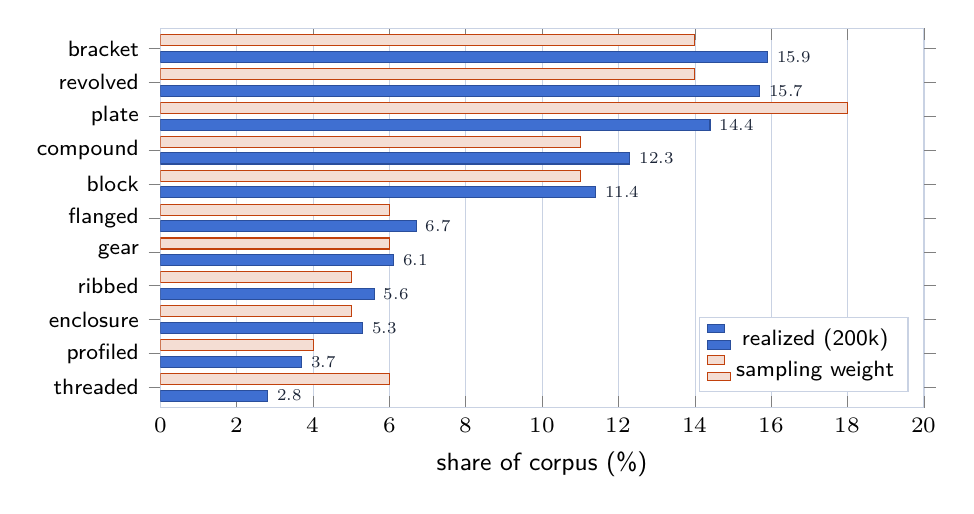
\begin{tikzpicture}
\begin{axis}[
  xbar, width=.93\linewidth, height=6.4cm,
  bar width=4pt, enlarge y limits=0.06,
  symbolic y coords={threaded,profiled,enclosure,ribbed,gear,flanged,block,compound,plate,revolved,bracket},
  ytick=data, y dir=normal,
  xmin=0, xmax=20, xlabel={\sffamily\small share of corpus (\%)},
  tick label style={font=\sffamily\footnotesize},
  label style={font=\sffamily\small},
  xmajorgrids, grid style={rule, very thin},
  axis line style={rule},
  legend style={at={(0.98,0.04)}, anchor=south east, font=\sffamily\footnotesize,
    draw=rule, fill=white},
  nodes near coords, every node near coord/.append style={
    font=\sffamily\fontsize{6}{7}\selectfont, color=ink, /pgf/number format/precision=1,
    /pgf/number format/fixed, /pgf/number format/fixed zerofill},
  ]
\addplot[draw=accentd, fill=accent] coordinates {
  (15.9,bracket) (15.7,revolved) (14.4,plate) (12.3,compound) (11.4,block)
  (6.7,flanged) (6.1,gear) (5.6,ribbed) (5.3,enclosure) (3.7,profiled) (2.8,threaded)};
\addplot[draw=accent2, fill=accent2!18, nodes near coords=] coordinates {
  (14,bracket) (14,revolved) (18,plate) (11,compound) (11,block)
  (6,flanged) (6,gear) (5,ribbed) (5,enclosure) (4,profiled) (6,threaded)};
\legend{realized (200k), sampling weight}
\end{axis}
\end{tikzpicture}
\caption{Realized family distribution on the 200k corpus vs.\ the configured
sampling weights. Realized shares drift below weight for low-diversity families
(\fm{threaded}, \fm{profiled}) because dedup removes saturating repeats, and
above weight where tier clamps add parts (\fm{bracket}). All weights are tunable
in \code{configs/default.toml}.}
\label{fig:dist}
\end{figure}

\subsection{Distribution}
\Cref{fig:dist} shows the realized family mix; complexity
tiers on the same corpus land at \textbf{11.0\%}/\textbf{49.6\%}/\textbf{30.3\%}/%
\textbf{9.0\%} for tiers 0--3, reflecting the per-family tier clamps that pull the
bare-primitive share down from its nominal 25\%. These are characterization
numbers, not targets; every knob is exposed in config.

\subsection{Formats and the size ladder}
The corpus is published on the Hugging Face
Hub~\cite{huggingfacedatasets} as a size ladder---\code{1k}, \code{2k}, \code{5k},
\code{10k}, \code{20k}, \code{50k}, \code{100k}, \code{200k}---each in six content
configs (\cref{tab:configs}) so a consumer fetches only what they need, from a
few-megabyte code-only pull to full geometry. Code-only data is JSONL with the
parametric \code{source} and \code{params} inlined; geometry configs are
Snappy-compressed Parquet with typed binary columns (\code{render\_*} images,
\code{stl\_bytes}, \code{step\_bytes}). Each config is also published restricted to
tiers~0--2 (a \code{-t0-2} suffix) for consumers who want to exclude the most
complex parts.

\begin{table}[h]
\centering\small\setlength{\tabcolsep}{6pt}
\renewcommand{\arraystretch}{1.12}
\begin{tabularx}{\linewidth}{@{}l X l@{}}
\toprule
\textbf{Config} & \textbf{Contents} & \textbf{Format}\\
\midrule
\code{<tag>}          & CadQuery \code{source} $+$ metadata $+$ \code{params} & JSONL\\
\code{<tag>-renders}  & $+$ eight-view render images                          & Parquet (image)\\
\code{<tag>-stl}      & $+$ binary STL mesh                                   & Parquet (binary)\\
\code{<tag>-step}     & $+$ binary STEP B-rep                                 & Parquet (binary)\\
\code{<tag>-geo}      & $+$ renders $+$ STL                                   & Parquet\\
\code{<tag>-full}     & $+$ renders $+$ STL $+$ STEP                          & Parquet\\
\bottomrule
\end{tabularx}
\caption{Six content configs per size \code{<tag>} (plus a tier-limited
\code{-t0-2} variant of each). \code{load\_dataset("jacobjennings/cadquarry",
"50k-full")} pulls everything for the 50k corpus; \code{"50k"} alone pulls just
code and metadata.}
\label{tab:configs}
\end{table}

% ===========================================================================
\section{Performance}\label{sec:perf}
% ===========================================================================
Generation validates every part by execution. Importing
the CadQuery/OCP kernel ($\sim$1--1.5\,s) is a fixed startup cost that CadQuarry
amortizes with a pool of \emph{persistent} workers that import once and then
build many parts each, fanning work across cores while keeping the
accept/dedup decision in strict attempt order---so output is independent of
worker count. Under the full default configuration, end-to-end throughput is
paced by the three solver-built mechanical families (\fm{gear}, \fm{threaded},
and \fm{tapped}, $\sim$14\% of the mix), which solve real involute/thread
geometry at a meaningful fraction of a second per part; the primitive families
alone build in milliseconds. \Cref{tab:perf} reports wall-clock times for
execution-validated generation (no geometry export); throughput settles at
$\sim$8--10 validated parts/s and climbs slightly with corpus size as the worker
warm-up amortizes.

\begin{table}[h]
\centering\small\setlength{\tabcolsep}{10pt}
\renewcommand{\arraystretch}{1.1}
\begin{tabular}{@{}r r r@{}}
\toprule
\textbf{Parts} & \textbf{Time} & \textbf{Throughput}\\
\midrule
1{,}000   & 2\,m 10\,s   & 7.5 parts/s\\
2{,}000   & 3\,m 30\,s   & 9.5 parts/s\\
5{,}000   & 9\,m 30\,s   & 8.7 parts/s\\
10{,}000  & 18\,m 45\,s  & 8.9 parts/s\\
20{,}000  & 36\,m 30\,s  & 9.1 parts/s\\
50{,}000  & 1\,h 30\,m   & 9.2 parts/s\\
100{,}000 & 2\,h 50\,m   & 9.8 parts/s\\
\bottomrule
\end{tabular}
\caption{Generation time on an AMD Ryzen Threadripper 9960X (24C/48T) with the
default 24-worker pool, full default config (mech families included),
execution-validated and geometry export excluded. The optimal worker count is
system-dependent and memory-bound at the largest sizes, so on machines with less
RAM fewer workers than cores may be needed to avoid swapping.}
\label{tab:perf}
\end{table}

% ===========================================================================
\section{Developer Experience and Community}\label{sec:dx}
% ===========================================================================
CadQuarry is meant to be inspected and extended, not just downloaded.

\textbf{No-install preview.} A 1{,}000-part sample is committed to the repository
and served as a self-contained in-browser gallery (Three.js, lazy-loaded
geometry) via GitHub Pages, so anyone can inspect the format and the real
geometry without installing anything.

\textbf{Live customizer.} \code{cadquarry serve} opens any part in a browser
customizer: move the sliders defined by \code{PARAMS} and the 3D view updates in
milliseconds---no regeneration, no ML---directly demonstrating the parametric
contract. The same tool browses a generated corpus as a filterable gallery.

\textbf{One-command pipeline.} \code{build} generates and exports every size in
the ladder; \code{publish} packs and uploads them as Hugging Face configs;
\code{build\_sample} refreshes the committed preview. Builds are resumable and
secrets (the HF token) are read from the environment and never logged or
committed.

\textbf{Versioned generator for community improvement.} Because the corpus is a
function of the generator and a seed list, contributions compose cleanly: a new
family or a fixed sampler becomes a new generator version with its own seed list
entry, and anyone can reproduce or extend a corpus without a hosted service in the
loop. The generator is \apache{}; there is no proprietary pipeline to reverse.

% ===========================================================================
\section{Generative-AI Disclosure}\label{sec:ai}
% ===========================================================================
\begin{warnbox}
\textbf{The dataset is not AI-generated.} Every part is produced by deterministic
procedural code and an exact geometry kernel; no language or diffusion model
samples, edits, or selects any geometry. This is a defining difference from
LLM-/diffusion-generated CAD: CadQuarry's outputs are reproducible from a seed and
validated by execution, not sampled from a learned distribution.

\smallskip
\textbf{The tooling was built with AI assistance.} The generator and supporting
code were developed by the author in collaboration with AI coding
assistants, under the author's direction and review; this is recorded in the
project's commit history. All
behavior is covered by an automated test suite and, for geometry, by the
execution-validity guarantee described in \cref{sec:valid}.

\smallskip
\textbf{This manuscript} was drafted with AI assistance and edited and verified by
the author, who is responsible for its content.
\end{warnbox}

% ===========================================================================
\section{Intended Uses, Limitations, and Licensing}\label{sec:uses}
% ===========================================================================
\textbf{Intended uses.} Pre-training and evaluation for CAD code generation and
program synthesis; point-cloud/mesh/multi-view $\rightarrow$ program recovery
(à la CAD-Recode~\cite{cadrecode}); text-conditioned generation and captioning
using the per-part plain-English dimension summaries (à
la Text2CAD~\cite{text2cad}, but with deterministic, reproducible descriptions);
parameter inference and customizable-part research that exploits the
\code{build(p)} interface; and geometry-quality studies using the structural
metrics that recent work emphasizes~\cite{cadmium}.
The multi-format ladder supports both lightweight code-only and full-geometry
workflows.

\textbf{Limitations.} The vocabulary, while broad, is mechanical-part oriented and
does not cover free-form/organic surfaces; tapered pipe threads (NPT/BSPT) are a
documented future addition, not a present capability; solver-built families are
byte-reproducible only against pinned \code{mech} versions
(\cref{sec:mech}); and the distribution reflects our sampling choices, which
consumers should re-weight as needed via config. The procedural design space is
ours, so the corpus is not a substitute for the long tail of real-world,
human-authored designs.

\textbf{Licensing.} Generator source is \apache{}; all generated
data---programs, STEP, STL, renders, parameter schemas, and metadata---is
dedicated to the public domain under \cc{}. The split is intentional and
unambiguous: do anything with the data, commercial use included, with no
attribution required. The two homes (an \apache{} GitHub generator, a \cc{}
Hugging Face corpus) map the code/data license boundary onto the platforms.

% ===========================================================================
\section{Conclusion}
% ===========================================================================
CadQuarry is a small contribution with a clear shape: a public-domain corpus of
\emph{parametric}, executable CAD programs, a raised complexity ceiling that
includes freeform sketches, lofts, sweeps, and real gears, threads, and tapped
holes, an unambiguous license, and a reproducible,
fast, inspectable generator. We hope the parametric-by-construction framing and
the \cc{} dedication make it a comfortable default for CAD-program learning, and
that the versioned generator invites the community to extend the design space
rather than re-scrape it.

\printbibliography

\end{document}
